\documentclass[10pt,twoside,dutch,english]{report}

    \usepackage[helvetica]{quotchap}   % fancy chapter beginning, times is other option
    \usepackage{fancyhdr}
	\usepackage[justification=raggedright, font=small, labelfont=bf,singlelinecheck=false]{caption}     %better control over captions (sideways, font, ...)  
    \usepackage{subfigure}  % with scriptsize or so, one can adapt the size


    \usepackage{enumerate}  % to make it possible to define the numbers (A,a, ...)
   % \usepackage{psfrag}
    \usepackage{graphicx}
    \usepackage{float} %fix floats on place you want (H)
    \usepackage{subfigure}
    %tables
    \usepackage{tabu} %table package. Veel mogelijkheden, bomen en bos
    \usepackage{longtable} % voor tables die langer zijn dan 1 pae
    \usepackage{mbenotes}
    \usepackage{tabularx}

 \usepackage{gensymb} %bijvoorbeeld graden symbool
 
    \usepackage{threeparttable} %tables with notes
       \usepackage[referable]{threeparttablex}
    %\usepackage[table]{xcolor}
  
	 \usepackage{booktabs}
   \usepackage{array}
  

    
    
    \usepackage{csvsimple} % csv inladen. Werkt nog niet
    %\usepackage{datatool}
    \usepackage{hyperref}
    \hypersetup{
    	colorlinks,
    	citecolor=dimgray,
    	filecolor=black,
    	linkcolor=black,
    	urlcolor=black
    }
    \definecolor{dimgray}{rgb}{0.41, 0.41, 0.41}
    
    \usepackage[toc,page]{appendix}
    
   % \usepackage{chappg}     % page numbering (chapno-pageno), for ToC
    \usepackage{url}        % for better url typesetting
    \usepackage{hhline}     % generates nicer table lines (without missing pixels) + more flexible
    \usepackage{afterpage}  % adds \afterpage command, which makes it possible to issue \afterpage{\clearpage} which flushes all floats after this page
    
    \usepackage[version = 3]{mhchem}     % use \ce {}  for chemical forumals
    \usepackage[a4paper]{geometry}
    \usepackage{fullpage}
   %\usepackage{cmbright}

    % \usepackage{microtype} %geeft nog een error
\usepackage[scaled]{helvet}
\renewcommand\familydefault{\sfdefault} %nodig voor helvetica
\usepackage[T1]{fontenc} %afbreken woorden enzo
\renewcommand{\baselinestretch}{1.3} %lijn afstand instellen
   \usepackage[round]{natbib}

\author{Job de Pater}
\title{Nitrogen mineralization for grassland soils } % was eerst anders.

\begin{document}



\setcounter{tocdepth}{1}
\linespread{1.0}
\tableofcontents
\linespread{1.3}
\thispagestyle{empty}
\pagebreak
\pagenumbering{arabic}

%\chapter*{Summary}

%\chapter*{Preface}

\chapter{Introduction}
%Voor 80% af op 10/7/15
The goal of this project is to get more insight in soil processes that influence the relation between soil characteristics, nitrogen mineralization and forage production. The focus of this study is not really on the outcomes, but more on the general pattern of analyzing. We will show the potential of this concept to be used and give some recommendations for improvement of this method. 

\section{Relevance: upgrade fertilization recommendations}
	We want to grow more forage with less fertilization. Nitrogen (N) is often growth limiting, partly because of the more and more strict regulations on fertilizer and manure application. Mineralization of soil organic matter (SOM) is a key soil process, a.o. because it provides the plants with mineral N. To maintain yields and prevent losses (leaching, volatilization) a balanced nutrient management is required. It is increasingly important to give farmers clear soil management guidelines. Much is known on the nutrient behavior in soils. However, relations between soil indicators and forage production are still vague.  This linkage has to be investigated to upgrade soil N fertilization recommendations and to better understand the SOM behavior. 
	
\section{Background: soil nutrient management}
%De aanleiding voor het onderzoek
	
			
		\subsection{Nutrient flows in grass production}
		The efficiency of forage production in terms of nutrient in- and outputs becomes more and more important in modern dairy farming. Forage production depends among others on soil quality, fertilization and other pasture management actions. It is known that fertilization practices affects the quality and composition of herbage directly, but there are not much studies that links soil fertility with herbage quality under practical conditions \citep{Reijneveld2014}. In terms of farm nutrient management, the aim is to  distribute the available amount of fertilizer and manure optimally. Therefore, the nutrient usage as well as the SOM mineralization has to be considered over time. It will also pay of in nutrient use efficiency to consider spatial soil differences of farms in order to optimize nutrient  distribution over all fields within a farm.  A first step is the development of the instrument Annual Nutrient Cycling Assessment (ANCA, dutch: 	\href{http://www.wageningenur.nl/nl/show/KringloopWijzer-2.htm}{\textit{Kringloopwijzer}}). The ANCA instrument is developed to presents a clear overview of individual farm nutrient cycles \citep{Aarts2013}. The ANCA model is a monitoring instrument that takes into account all possible nutrients flows. All fluxes can be described by existing data of the whole farm (Figure \ref{fig:KLW}). This tool has high potential for governmental regulations, farm management advice and it provides knowledge and data for fundamental and applied research. However, a disadvantage of the ANCA system is that the soil part is not yet implemented. It is not fully understood in what extend soil processes have influence on for example leaching or crop uptake under certain circumstances.  For optimal dairy farm soil management, the ANCA model is useful when the tool is linked to management practices. 
        
      		\begin{figure}[ht]
			\centering
			\includegraphics[width=0.6\linewidth]{intro_KLW}
			\caption{The different parts of the ANCA instrument: animal, forage, milk, fertilization and soil. Data for the instrument is provided by certain companies. The relations between fertilization, mineralization and crop yield are still insufficient understood. Source: \citet{Holster2013}. }
			\label{fig:KLW}
		\end{figure}
		
		\subsection{Bottom-up innovation in the dairy chain}
		 It is essential to implement research knowledge into practice when progressively innovation is the purpose. An applied and farm based approach is required, where communication with the farmers is of high importance. An example of an applied research approach is the project "Praktijkaanpak 'verborgen rendement uit de bodem'", which is a.o. conducted by NMI. The aim is to utilize soil properties that are yet not used or still unknown by the farmers. This will be done by introducing a field based fertilization plan, which takes in mind the production aim, soil fertility and the actual weather conditions. Such approach can stimulate farmers to close their nutrient cycles and it provides knowledge which helps us understanding soil plant interactions. 
		
	\section{Objectives}
			In this project I want to identify and evaluate relationships between given soil parameters and the N mineralization in soils.
			
			
			My objectives are:
			\begin{itemize}
				\item   To calibrate and validate a descriptive model for the prediction of N mineralization. I will give possible explanations for the observed outcomes using literature.
				\item	To come up with practical implementations in practice. I will evaluate the applicability of the relevant indicators and relations.
				
			\end{itemize}
			
			Significant and relevant interactions between soil fertility, N mineralization and forage production could only be identified when large data sets are available. In this project I will give a proof of concept where I will show a general pattern of how such study approach could be conducted. 
			

\chapter{State of the art} % Hoever zijn we in het onderzoek gekomen. Formuleren van nieuwe onderzoeksvragen
	\label{chap: state of the art}


\section{Soil fertility on dairy farms} 
Soil fertility changes over time due to shifts in fertilization and soil management practices \citep{Hanegraaf2009}. Soil fertility is highly related to the organic matter content. The SOM content and quality is directly related to physical, chemical and biological soil functionality. The quality of SOM depends on its stability and composition what on its turn determines how fast the SOM is decomposed by soil microorganisms. There are many studies on the mineralization of SOM and on the N dynamics in soil \citep{Wander2004, Haynes2005, Ros2011}. However, yet clear relationships between SOM nutrient supply and other soil indicators remain elusive. N dynamics in soil plant relations varies between weather conditions and are difficult to study because N is available is many forms in the soil environment \citep{Nannipieri2009}. Hence, direct relations between SOM content and forage production are yet still unknown or vague \citep{Hanegraaf2009}. \citet{Reijneveld2014} suggested that relationships between soil characteristics and herbage quality may become more clear when linkage at field level can be made between soil and herbage characteristics. 

\section{Predicting N supply }
\subsection{N mineralization}
Understanding N mineralization is essential to provide optimal fertilizer recommendations for the highest N utilization. N mineralization is the conversion of organic N to \ce{NH4+} and is done by soil microbes.  This influence the amount of the for plants available N in soil \citep{Myrold2008, Geisseler2010}. Soil microbes influence SOM cycling not only via decomposition but also because microbial products are themselves important components of SOM. Mineralization is almost always accompanied by immobilization of N \citep{Powlson1993}. We mean net mineralization when talking about mineralization. 

In general, N mineralization over time for a certain amount of soil  follows the curve showed in Figure \ref{fig:intro_Ncum}. Three characteristics of this curve are important. 
\begin{enumerate}
	\item The mineralization rate at the start of the decomposition. Decomposition rates depend on the resource quality (how stable), characteristics of the decomposing organisms (e.g. C/N ratio) and environmental conditions (e.g. weather, mineralogy) \citep{Lavelle1993}. 
	\item The potential N mineralization. This is the total N mineralized at equilibrium. The potential total N mineralization depends on the capacity and ability of the microbes to decompose the different fractions of SOM (ref)
	\item The time it takes to reach the potential N mineralization(1). This depends mainly on the initial mineralization rate (ref).
\end{enumerate}


\begin{figure}[h]
	\includegraphics[width=1\linewidth]{intro_Ncum}
	\caption{The nitrogen mineralization curve with its characteristics. The three important characteristics are the mineralization rate at start of the mineralization (1), the potential mineralizable N (2) and the time to reach the potential mineralizable N (3). These characteristics determine the decomposition of SOM}
	\label{fig:intro_Ncum}
\end{figure}

Despite the fact that OM plays an important role in decomposition and nutrient supply, OM is not a good indicator for soil fertility in the field \citep{Hanegraaf2009}. Changes in OM content take place gradually and subtle, so small changes are difficult to detect \citep{Ghani2002, Hanegraaf2009}. Total (potential) N mineralization (Figure \ref{fig:intro_Ncum}, (2)) is linked with the SOM content since the SOM provides the mineralizable N. However, this does not tell us anything about the mineralization rate (Figure\ref{fig:intro_Ncum}, (1)), which give a better measure for the short term.  A preferred indicator would be the labile fractions of the organic pool, such as the easy biodegradable and extractable fractions, as shown in Figure \ref{fig:intro_haynes} \citep{Haynes2005}. Those fractions are measurable parts of organic matter and not the theoretically defined pools of SOM \citep{Wander2004}. Several studies observed significant relationships between EOM fractions and the soil N mineralization \citep{Ros2011a,Ros2012}.  They concluded that for different studies distinct EOM fractions are identified as the best predictor of mineralizable N, depending on presumably the regions, years, seasons, land uses and variations in the analysis reproducibility of extraction methods \citep{Ros2011}. This suggests that the search for the best predictor of mineralizable N cannot be fulfilled by statistical analysis alone, and emphasize the need for studying the underlying mechanisms \citep{Ros2011}. 

	\begin{figure}[h]
		\includegraphics[width=1\linewidth]{intro_haynes}
		\caption{Schematic overview of the relationships between various organic matter fractions. Source: \citet{Haynes2005}.}
		\label{fig:intro_haynes}
	\end{figure}

The classical paradigm is that SOM stability mainly depends on molecular structure of organic material (resistance to breakdown) and humus formation (by condensation reactions). A new view is developing, suggesting that not only organic matter quality but also other factors strongly determine decomposition \citep{bingham2015}. The resistance to decomposition is regarded as a property which is controlled by environmental factors such as microbial inhibition and distribution and also physical/chemical protection and disconnection \citep{Lutzow2006,Schmidt2011}.


\subsection{Possible indicators for usage in practice}
A soil indicator that can be used in practice for the prediction of N mineralization should met some requirements. \citet{Gil-Sotres2005} appointed the following criteria. The indicator should preferably measure more than only one soil function and should be sensitive to changes in short term. Additionally, target and critical values should be known for the indicator. And last but not least, the implementation of the indicator in practice should be easy, which means it should be simple to analyze with low costs. 

Literature shows that the biological available N pool is related to a.o. the following  measurable indicators that are relevant for practical usage. This are both indicators for estimating the pool size as well as measures for the N flux through the different pools.

\begin{itemize}
	\item \textbf{Hot water extractable carbon (HWC)}. HWC is the organic carbon fraction that is extracted with hot water. The dissolved organic carbon (DOC) fraction, that is initially in the solution, is excluded by first extracting with cold water.  The HWC is strongly related to labile OM and microbial biomass\citep{Ghani2002, Ghani2003}, where labile OM is seen as the OM that has a turnover time of a few days up to some weeks. HWC could possibly be measured with the NIRS methodology \citep{Vasques2009}, hence it could be implemented in routine labs. 
	\item \textbf{Extractable organic nitrogen (EON)}. Organic N can be extracted by for example hot water, \ce{KCL}, \ce{CaCl2}, \ce{HCL} or other solutions. EON can be an indicator of microbial activity (and so mineralization) \citep{Schimel2004}. It should be noted that probably the flow of N through the dissolved organic N (DON) pool controls the rate of mineralization more than its size; the fluxes could be high, also when the DON pool is small. Big disadvantage of this approach is that EON concentration measurements highly depend on methodology \citep{Ros2009}. 
% * <jobdepater@gmail.com> 2015-09-16T10:25:47.136Z:
%
%  Klopt niet, nog aanpassen. Schimel zegt wat anders
%
	
	\item \textbf{Potential nitrogen mineralization (PNM)}. The PNM is an \textbf{aerobic mineralization} analysis method. The PNM is defined as the total mineralized N over 12 weeks or the rate of mineral N production over the 12 weeks (slope of cumulative Nmin curve, see Figure \ref{fig:intro_Ncum}) of the aerobic incubation. Numerous methods have been developed, what is nicely described by a.o. \citet{Doran1996} and \citet{Canali2005}.
	
	\item \textbf{Biological fertility indicator (BFI)}. The BFI is the \textbf{anaerobic mineralization} analysis method. The BFI is defined as the total mineralized N in 7 days under anaerobic conditions.
	
	\item \textbf{Soil respiration (Resp)}. Respiration is closely associated with life \citep{Bloem2005}. Soil respiration is measured as \ce{CO2} production and \ce{CO2} release indicates  that at the same time \ce{O2} is taken up. This occurs when the environment is aerobic. This Respiration is done by the micro organisms and can be defined as the uptake of \ce{O2} while, at the same time, \ce{CO2} is released \citep{Bloem2005}. The N mineralization is coupled with the \ce{CO2} release \citep{Geisseler2009}. (??? uitleggen). 
	
	\item \textbf{Microbial biomass (C-mic)}. Microbial biomass has a high turnover rate, so it is suggested to be a sensitive indicator of changes in tillage systems \citep{Lynch1980, Sparling1997}. It is also related with soil physical characteristics \citep{Schimel1986}. A downside of this indicator is the difficulty of the measurement, but \citet{Sparling1992} suggested HWC and \citet{Myrold1987} suggested the PNM as a good approximation of the microbial biomass. 
	
	\item \textbf{Ratios} such as C/N ratio, fungi/bacteria, HWC/C-total, PNM/C-total, C-mic/C-total. This ratios can be indicators for the stability (biodegradability) of the organic material in the soil \citep{Sparling1992, Hanegraaf2009} and the intensity the agricultural system \citep{Bloem2004}
	
\end{itemize}
		
	There are various techniques for predicting biological available N \citep{Haynes2005}. It can be done by chemical extraction methods or biological incubation methods, but none of these methods is universally accepted \citep{Nannipieri2009}. The mineralization can be simulated in relation to abiotic soil properties or biological indicators. The potential N supply over a period could be predicted by simulation models which are widely available \citep{Manzoni2009}. A nice example is the MINIP model \citep{Janssen1984}, which is used in the Netherlands in several tools for soil management recommendations. Those mineralization models are refined over time for research and for practical usage \citep{Yang2000,Postma2004}.  However, those models are not used in the Netherlands for prediction the mineralization on grassland soils. This is probably because it is difficult to calibrate the models for each specific field due to the heterogeneity of the fields \citep{Ros2015}. 
		
\subsection{Current N recommendations in the Netherlands} % Hanegraaf Zand rapport
Currently, most standard soil management advises for farmers consists of general analyses concerning nutrient amounts in the soil. At present, in the Netherlands, the fertilizer N recommendations of grasslands are build on the Non Fertilizer N Supply (NFNS, Dutch: NLV), which is based on the work of \citet{Hassink1995a}. The NFNS is defined as the N uptake on unfertilized plots and is calculated by regression models based on the organic N content in the top 0-10 cm soil layer \citep{Bemestingscommissie2012}. The NFNS does only superficially take into account the different biodegradability of the SOM pools and environmental conditions. The predictions seem not to be accurate for today measurements, as shown for example in Figure \ref{fig:intro_ros}. Deviations from the NFNS predictions are up to 100 kg N per ha, so the farmer does not get fully insight in the potential of the soil to make nutrients free for plant uptake. Hence, it is recommended to upgrade the current fertilizer N recommendations \citep{Hanegraaf2009, VanEekeren2010, Ros2015}. Another issue is that for the fertilizer N recommendations for both grassland and arable soils the same name (NFNS) is used, while different protocols are carried out. For arable soils the recommendations are based on the MINIP model of \citet{Janssen1984} and soil samples are taken from the 0-20 cm soil layer (tilling depth). (\textbf{Waar? uitleg..})\\
%review NLV: Bussink 2002
%weer: Ros&Bussink 2012

		\begin{figure}[t]
			\includegraphics[width=1\linewidth]{intro_ros}
			\caption{Relation between N-total and the predicted N supply (NFNS) compared with data from experiments on sandy soils. The accuracy of the predictions is currently still too low. Note that the data comes from samples from the 0-20 cm soil layer (normally the samples for grassland soils comes from the 0-10 cm layer.) Source:   \citet{Ros2015}, data confidential.}
			\label{fig:intro_ros}
		\end{figure}
		
\subsection{N recommendations in other countries}
European countries have more of less fixed N-application standards (maximum allowable N rates) per crop or crop group \citep{VanDijk2009}. Constraints are given in the Nitrates Directive of 1991 (ref). Each member state have to define Codes of Good Agricultural Practice. N recommendations are the bases of a good fertilizer planning. However, it is difficult to compare all fertilization recommendations, because they depend on many factors


USA: Illinois Soil Nitrogen Test (ISNT)...measures a soil's ability to slowly provide nitrogen to the crop during the growing season.

\subsection{Future}
 In the ideal situation the farmer knows what amount of N is available for crop growth at each time period, so he can adjust fertilization rates on the grass requirements. Therefore, other variables that influence the N mineralization, such as weather conditions and SOM related characteristics and other variables (e.g. textural properties) should been considered in prediction models \citep{Ros2015}. The N fertilization recommendation tool \textit{'Dynamic N Advice'}, which is under construction by NMI, is an attempt to take into account the weather conditions.  It makes usage of location based weather predictions (KNMI data), an updated version of the NFNS advice, the mineralization model MINIP, a simple grass growth model and district averages of soil characteristics (BLGG data). A data flow scheme of the Dynamic N Advice can be found in Appendix \ref{chap: dynN}.



	
	
	
	

\chapter{Materials and methods}

A existing data set is analyzed for statistical relations between biotic and abiotic soil properties in order to predict soil N mineralization. This relationships were validated with data from field experiments, where grassland soils were analyzed for several key indicators. 

\section{Calibration data: internship Echeverri}
The calibration data is provided by the internship work of  \citet{Echeverri2014}. In his project he tested the following three methodologies to assess SOM quality. 1: Validation of  HWC methodology to predict the biologically decomposable SOM in short term. 2: Understanding SOM pathways by performing incubation and SOM fractionation. 3: Providing insight about thermogravimetric analyses in SOM study.  He suggested that hot water extractable carbon HWC extracted the most labile carbon fraction of soils and therefore he assumed HWC to be an appropriate indicator of SOM decomposability in short term.

For his study Echeverri analyzed 21 soil samples from different agricultural fields in the Netherlands. Soil types differed in SOM and clay content. 
The available data consist of the following analyses. 

	\begin{enumerate}
	\item \textbf{Standard soil parameters} \\
	This data consists of near infra red spectroscopy (NIRS) analyses and classical analyses, both conducted by the lab of \href{http://blgg.agroxpertus.nl/}{\textit{BLGG AgroXpertus}}. This analysis contains about 60 soil parameters that are used in the extensive soil management advices (the BLGG \href{http://blgg.agroxpertus.nl/product/bemesting/bemestingswijzer-bouwland}{\textit{'Bemestingswijzer'}}). 
	
	\item \textbf{Mineralization indicators}\\
	Soil life indicators are used to give a measure of the activity of the soil live. Microbial activity is often linked to the potential quantity of N that can be mineralized. 
	\begin{itemize}
		\item The potential nitrogen mineralization (PNM).  Units: mg N kg $^{-1}$ per day. The data of \citep{Echeverri2014} shows only significant values for \ce{NO3}, because all concentrations of \ce{NH4} were below the detection limit. 
		\item The biological fertility indicator (BFI). Units: mg N kg $^{-1}$. Measurements were done on field moist soils (BFI-m) and on dried soils (BFI-d). 
	\end{itemize}
	
	\item \textbf{HWC} \\
	HWC is calculated as the difference between the inorganic and organic carbon after hot water extraction. Units: mg C kg $^{-1}$.   
	
	\item \textbf{Potential soil respiration rate (Resp)}\\
	The soil microbe respiration is measured as \ce{CO2} production at optimum moisture and temperature. Units: mg C kg $^{-1}$ h$^{-1}$.   
	%add some more information
\end{enumerate}

All data of Echeverris study can be found in Appendix \autoref{chap: Calibration data}. This data is used for calibrating the statistical models for predicting N mineralization.  

Possible indicators for the prediction of N mineralization that are measured for the calibration data are the PNM, HWC, Resp and the BFI. The opportunity for introduction of mineralization indicators in practice depends on the accuracy and precision of the measurements and how easy it is to automate the analysis of the indicator to make routine determinations more efficient. Hence, both HWC and BFI seems to have the most positive perspectives to be implemented into fertilization advisement tools, because the possibility to measure these indicators with the NIRS method \citep{Hanegraaf2008, Vasques2009}. 

% A short study is conducted on the performance of different BFI methodologies (Appendix \ref*{chap:bfis}). 


\section{Validation data: grassland soils Friesland}
The statistical models are validated with data that is collected from dairy farms that also join the NMI project "Verborgen rendement uit de bodem". For this project it was possible to analyze the soil for PNM (anaerobe), BFI (anaerobe) and HWC   as indicators for the N mineralization. 

All validation data can be found in Appendix \autoref{chap: Validation data}.

\subsection{Field selection and sampling}
Soils were collected from grassland soils at four dairy farms in Friesland (Table \ref{tab:results_farms} ). The chosen fields are also used for other research of NMI on the dynamic spatial and temporal nitrogen behavior. All fields ranged from 2.5-5.3 ha and consists of sandy soils, with some loamy characteristics. %misschien meer over zeggen? 

\begin{table}[ht] %Table Field information
	\caption{Field information and soil characteristics of the top layer (0-10 cm) for the growing season of 2015 (Sampling on 06/16/2015) }
	\footnotesize 
	\renewcommand{\arraystretch}{1.2}
	
	
	\begin{tabu} to \textwidth{@{}X[c]X[l]X[l]X[c]X[l]X[l]X[l]@{}}% {@{}rrrrrrr@{}} 
		\toprule	\rowfont{\bfseries}
		Farm & Place & Location & OM (\%) & Clay (\%) & Ntot (mg/kg) & pH \\  \midrule
		A & Olderbekoop & Lat: 52.94 Lon: 6.13 & 8.4 & 3 & 3990& 5.6 \\
		B & Olderbekoop& Lat: 52.93 Lon:6.11 & 4.5& 2& 1670& 5.8\\
		C & Nijeberkoop & Lat: 52.96 Lon: 6.19 & 6.8& $<$1& 2820& 5.9\\
		D & Appelscha & Lat: 52.96 Lon: 6.42 & 7.3& 2& 2890& 5.6\\		 \bottomrule
	\end{tabu}
		\label{tab:results_farms}
\end{table}

Each grassland field was harvested several cycles and was alternately cut for silage and grazed. The initial protocol was that within a week before each cutting upward of the second cutting, we should have taken a sample of the fields \ref{fig:mm_samples} and subsequently analyze the samples for the indicators. Because of the diversity in farming methods (grazing or not) and differences in cutting times, we toke samples at fixed dates.  Even when grazing was applied, a sample was taken at the same time as it was done from the other fields. Samples were taken on 06/16/2015, 07/03/2015, 03/08/2015 and 04/09/2015. All samples were taken from the 0-10 cm top soil layer of each field. Per sample, $>$70 sub samples were taken in W-pattern. 

\begin{figure}[h] %Figure Sampling Time Plan
	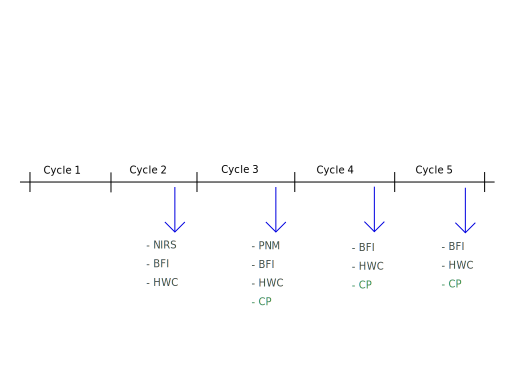
\includegraphics[width=1\linewidth]{mm_samples}
	\caption{Sample time plan of the Friesland samples. The first cycle was missed. From the second to the last cycle, the BFI and the HWC was measured. For the second cycle, the NIRS analyses was done. For the third cycle, the samples for the PNM analysis were taken. From the third to the last cycle, the herbage indicators were determined (relevant: crude protein (CP). }
	\label{fig:mm_samples}
\end{figure}

\subsection{Soil analysis methods}
Soil samples were mixed by hand and passed through a 5-mm sieve. Big roots and grass leafs are removed. The samples were stored field-moist at a temperature of 4 °C. Analysing methods are done within 10 days after sampling. 
The complete protocols used for the chemical and physical analysis are described in Appendix \ref{chap: Protocols}. In short the following procedures were done. 

\subsubsection{How water extractable carbon (HWC)}
The HWC was determined according to the method used by \citet{Ghani2003}. In this method the first step involved removal of readily soluble C from the samples. The second step was extraction of labile components of C at 80 \degree C for 16 h. This is referred to as hot-water extractable carbon (HWC).

\subsubsection{Aerobic N mineralization (PNM)}
The PNM was determined according to the protocol described by \citet{Ros2014}. Here the samples are incubated for 12 weeks under aerobic conditions and 20 \degree C. Mineral N was determined at 1, 3, 6, 9 and 12 weeks after start of the incubation. 

\subsubsection{Anaerobic N mineralization (BFI)}
The anaerobic mineralization incubation was conducted by the BLGG lab. The lab followed the procedure which is described by \citet{Hanegraaf2008} Here a anaerobic incubation of seven days was applied and thereafter the mineral N was determined. 
%zie book 



\section{Statistical analysis}
Data were analyzed with R (v. 3.1.3), using the RStudio IDE and a.o. the packages pls and the lm function. 
\subsection{Calibration}
Three data points were removed because they contained erroneous data ($PNM\leq 0$). This could be due to immobilization, but we assumed this to be errors. For the PNM, only validation data of \ce{NO3} is used, because accurate \ce{NH4} data were not available for the calibration data (all measured below  the detection limit). 

%All data of one parameter set are log transformed when necessary to met the normality requirements (test of \citet{Shapiro1965}). Parameter sets were not normally distributed when grouping them into soil types. 
Data of the classical soil analysis is used, because the NIRS analysis are based on the classical analyses. When data of the classical soil analysis was not available, data of the NIRS analysis was used. This was not completely possible for the organic carbon measurements, because not all data was available for both the classical and the NIRS analysis. For anaerobic mineralization, the BFI that was determined on moist samples (BFI-m) was used in the statistical analysis. 


Univariate partial least squares (PLS, as described in \citet{Mevik2013}) regression was applied on the data to get insight in the variation of the mineralization and to select the relevant parameters for the explanatory models. For explanation about PLS regression, we refer to the interpretation paper of\citet{Garthwaite1994}. 


Multiple linear models were made to predict the N mineralization on grassland soils. To get a first insight in the relative importance of the variables, a step wise regression was carried out which was based on the Akaike information criterion (AIC, \citep{Sakamoto1986}). The models were made by trial and error with the criteria that all parameter values should be significantly (\textit{p}<0.05) contribute to the model. For evaluating the validity of the models we use the coefficient of variation and the analysis of residuals. 

The best multiple linear model was chosen and calibrated for the whole data set as well as for only the mineral soils and only the sandy soils. 

\subsection{Validation}
The calibrated models were validated with the Friesland soil samples of the second growing cycle. All data is evaluated to see the difference between the observed and the predicted values.  To interpret the results for field situations,  the units of the mineralization rate are converted from $mg\: kg^{-1}\: day^{-1}$ to $kg\:N\:ha^{-1}\: month^{-1}$. This conversion was based on the assumption of a mineralization depth of 10 cm and a  bulk density $(\rho)$ which is calculated using the following formula\footnote{This formula to calculate the bulk density is being used in the BLGG routine lab. parameter values are: $a=0.02525, b=0.6541, c=0.00000067, d=0.00007792, e=0.00314712, f=0.06039523, g=1.33932206$. }:
\[\rho = if (Clay<8):\: {1/(a\cdot SOM+b)} \:\:else:\: {c\cdot SOM^4-d\cdot SOM^3+e\cdot SOM^2-f\cdot SOM+g}\]
$SOM$ and $Clay$ are expressed in percentages and were the average values of the available data. 

In addition, data from\citet{Ros2011} is used to inspect if the chosen model was also valid for data from other data sets. 


\section{Farm management -->naar appendix }
The heterogeneity of the soils was analyzed to give the farmers insight in the spatial soil characteristics within their fields. To do so, different samples were taken from characteristic field areas for each farm on 07/03/2015. 

In addition, for the second and the third grass cycle, an N fertilization advice was made for each farm, using the Dynamic N Advice tool (ref). Advice for the second cycle was given on 05/11/2015  and advice for the third cycle was given on 07/15/2015. Input values for the model can be found in Appendix \ref{chap: dynN}. When data was not available, the model used default values or district averages. All farms were in the same region (Table \ref{tab:results_farms}), and closest to the KNMI weather station in Marknesse, Flevoland. The crude protein (CP) was analyzed from fifth to sixth cycle (Figure \ref{fig:mm_samples}) to evaluate if the crop uptake according to what was expected. 



\chapter{Results}

The results shows that the N mineralization could be predicted by simple and multivariate linear models. However, the accuracy of the predictions is very low. etc... % prediction intervals were smaller when the model was calibrate only on the mineral soils. 
%-----------------------------------------------------------------------------------------------------------------------------------------------------------
\section{Data exploration}
%-----------------------------------------------------------------------------------------------------------------------------------------------------------
\subsection{Soil properties}
The soils of the calibration set are collected from agricultural fields from over the Netherlands. The 21 soils consists of different clayey, sandy and peaty soils. Hence, they varied widely in their physical and chemical characteristics (Figure \ref{fig:results_boxplots} and Table \ref{tab: results_char}). The key factors varied between 0.07 and 0.66 mg N kg $^{-1}$ d$^{-1}$ for the mineralization rate; between 239-5099 mg C kg $^{-1}$ for HWC and between 2.4 and 20.2 \% for OM. 

	\begin{figure}[ht] % boxplots van bodemeigenschappen
		
		\centering
		\includegraphics[width=1\linewidth]{results_boxplots}
		\caption{Boxplots of key soil mineralization indicators grouped on soil type: dalgrond (\textit{n=4}), dekzand (\textit{n=4}), kleiig veen (\textit{n=3}), river clay (\textit{n=3}) and sea clay (\textit{n=3}). It shows  that much of the variation could be explained by soil type}
		\label{fig:results_boxplots}
	\end{figure}
Figure \ref{fig:results_boxplots} shows the variability of the key indicators for soil N mineralization. Much of the variation could be explained by the differences in soil types. This shows the disadvantage of combining all data. 

\subsection{Soil indicators for N mineralization} 
In this study there are four different biological essays on the N supply that can be used as indicator for the N mineralization. They consists of the aerobic long term measurements on dried soils (PNM), the anaerobic measurements on dried soils (BFI-d), the anaerobic measurements on moist soils (BFI-m) and the NIRS measurement of the BFI-m (BFI-nir). We assume the aerobic PNM the best predictor of the real mineralization, because it approximates the field conditions the most. Hence, the PNM is used as response variable. 

 \subsubsection{Aerobic mineralization rate as response variable} 
During the 12 weeks aerobic mineralization, the cumulative mineral N (here \ce{NO3}) increased on average up to 35 mg kg$^{-1}$ for all soils (Figure \ref{fig:results_Ncum}). Cumulative mineralization was the highest for peaty soils (47 mg kg$^{-1}$) and the lowest for clayey soils (24 mg kg$^{-1}$).  In the 12 weeks incubation period, we assume the N mineralization to be still in the linear phase (see also Figure \ref{fig:intro_Ncum}). Subsequently, we consider the slope of the cumulative N mineralization curve as an indicator for the N mineralization. The mean mineralization rate  is 0.17 mg N kg$^{-1}$ per day. Soil type had a strong effect on the mineralization rate: for sandy soils the average mineralization rate was 0.26 mg N kg$^{-1}$, for clay soils 0.14 mg N kg$^{-1}$  and for the peaty soils 0.34 mg N kg$^{-1}$. The variance was greatest for the sandy and lowest for the clayey soils. 

The soil indicators of the calibration data set shows various significant correlations (Figure \ref{fig:results_corr}), despite of the high variation in soil characteristics (Figure \ref{fig:results_boxplots}). As expected, in particular the indicators for labile organic matter (BFI, HWC, Resp) shows positive correlation with the aerobic mineralization rate (r > 0.77). Indicators for organic matter show somewhat less correlation with the aerobic mineralization rate compared with the anaerobe mineralization (BFI-n). Correlation plots for the variables of  only the mineral soils or only the sandy soils  show that the labile organic matter indicators are less correlated for the clayey soils compared with the sandy soils  (Appendix \ref{chap:corr}). Also, for the clay soils there is hardly (r = 0.3) any correlation between the PNM and N total. Remarkable is the  correlation between PNM and respiration, which is negative (r = -0.8)  for the clayey soils and the positive (r = 0.8) for the sandy soils. All correlation plots show a positive correlation between OM, N total and C total (r > 0.8). The peaty soils shows much strong correlations, however this s caused by the low number of peaty soils (n = 3) where one is deviating strong of the other two. The second component might be somewhat related to more physical characteristics of the soil (CN, Sand, C total). 
	\begin{figure}[h] %Correlatie matrix
	\centering
	\includegraphics[width=0.7\linewidth]{results_corr}
	\caption{Correlation matrix of all variables for the whole data set.  Red numbers denote negative and blue positive correlations. Lower color intensity indicates less correlation. Correlation plots for the variables of  only the mineral soils or only the sandy soils can be found in Appendix \ref{chap:corr}}.
	\label{fig:results_corr}
\end{figure}

PLS analysis showed that the variability of the PNM rate (mg N kg$^{-1} $ day$^{-1}$ ) is mainly explained by a component that is related to organic matter (Appendix \ref{chap:PLS}). Highest related indicators were HWC, respiration, C/N ratio, BFI, pH, Silt and CEC. This component explains about 32\% of the variability around the prediction of the PNM rate for the whole data set. The second explanatory component is probably related to more chemical-physical properties of the soils, though this were weak relationships and it only explains 9.1\% of the variability.  Total explained variability was not higher when only considering the mineral soils (component 1: 28\% and component 2: 17\%. However, when applying PLS regression only on the sandy soils, the explained variability increased a few percentage compared with the PLS regression applied on the whole data set. For the sandy soils, the first component explains 39\% and the second component explained 17\% 

\section{Model calibration}
In this section, a descriptive model for the prediction o f N mineralization is defined. As already mentoined, PNM was significant related to the indicators for labile organic matte indicatorsr: HWC, Resp and BFI where the direct relationship with OM was relatively poor. The relation between HWC, the mineralization rate and OM for the sandy soils is shown in Figure \ref{fig:results_pnm_hwc}.  Simple linear model plots of the other indicators for labile organic matter can be found in Appendix \ref{chap:Model output}.

	\begin{figure}[h] %pnm~hwc
	\centering
	\includegraphics[width=0.7\linewidth]{results_pnm_hwc}
	\caption{Relation between HWC and OM.  The blue lines denote the prediction interval. Triangle values show the validation values of the Friesland farms.}.
	\label{fig:results_pnm_hwc}
\end{figure}

Several significant  (\textit{p}$<$0.001) models were made for the prediction of the N mineralization rate. Table \ref{tab: results_mods} in the appendix shows some appropriate models for the prediction of N mineralization rate. For all models, the parameter estimates were significant and the adjusted coefficient of variation was $>$0.63. The standard errors of the prediction (SEP) were  relatively large compared with the mean mineralization rates, what was in line with the large standard deviation of the calibration data (sd = 0.17 mg kg$^{-1}$ d$^{-1}$).  According to the Akaike information criterion (AIC), which gives a measure of the relative quality of the different models, the models with one of Resp, HWC and C-tot included are preferred above the other models.  It especially turns out that addition of soil respiration in the multivariate approach ends up in more significant models what was expected since the correlation between respiration and the mineralization rate and the HWC (labile OM) was relatively high. The Bayesian information criterion (BIC), which is closely related to the AIC, gives about the same results. However, those criteria gives not a absolute measure of the models. 

Statistically, the best model was the one with Resp as main factor plus an interaction term between C-tot and sand. However, the only (suggestive) explanation could be the protection of SOM by the sand.  We do not have a convincing explanation for this interaction, so we reject the validity of this model. 

 The second best model we identified was the model were HWC is interacting with OM, what is an understandable interaction.  HWC is expected to be measured with the NIRS method in future \citep{Vasques2009}, so it can be implemented in routine labs. This is an advantage over respiration, which is quite difficult to analyze. For the above reasons, we choose model 8 for the validation. With the parameter estimates this model is: 
\begin{equation} %choossen model
Mineralization\  rate = a\cdot HWC +b\cdot OM +c\cdot HWC\times OM + d
\label{eq: model}
\end{equation}
The parameter estimates for HWC, OM, the interaction between HWC and OM and the intercept with corresponding p values are shown in Table \ref{tab:parameters}. The parameters were estimated for calibration on the whole data set, the mineral soils and the sandy soils. All parameters were insignificant for the  calibration on only the mineral soils or only on the sandy soils. Hence, for the subsets, simple linear models were used with either HWC or OM as explanatory variable. All models were significant (\textit{p}<0.001). For the simple linear models, the intercept term was added, also when the parameter estimate was not significant because of the practical meaning and interpretation. For this reason, the models are only valid within the range of the calibration data.  For none of the models, the intercept term was significant. Additional model (validation) output can be found in Appendix \ref{chap:Model output}.  

\begin{table}[h] %Table Field information
	\caption{Parameter estimates of the model (Equation \ref{eq: model})calibrated for all soils, only the mineral soils and only the sandy soils. Parameters were estimates for the effect of HWC (\textbf{a}), OM (\textbf{b}) and HWC$\times$OM (\textbf{c}). Intercepts (\textbf{d}) were not significant. All calibrations resulted in highly significant models (\textit{P}<0.001)}.
	\footnotesize 
	\renewcommand{\arraystretch}{1.2}
	
	
	\begin{tabu} to \textwidth{@{}X[1.2,l]X[c]X[c]X[c]X[c]@{}}% {@{}rrrrrrr@{}} 
		\toprule	\rowfont{\bfseries}
       										 & a \quad (HWC)	 &b \quad (OM)         &c (HWC$\times$OM)          						& R$^{2}$ model\\ \midrule
                                             
     Whole data set        & 1.96e-04(\textit{p} < 0.001)		 & 1.13e-02 (\textit{p} = 0.07)		& -5.87e-06 (\textit{p} = 0.04)		&0.93\\
     										
     Mineral soils             &&&\\
     \quad Option 1			& 0.028 (\textit{p} <0.001	)&$-$									&$-$									 					 				&0.68\\
     									
   \quad Option 2			& $-$	      						&	 0.028	(\textit{p} <0.001)		&$-$																	&0.68\\
     	
 
      Sandy soils             &&&\\
     \quad Option 1			& 2.177e-04 (\textit{p} < 0.001)	&$-$									&$-$									 								&0.93\\
     				
   \quad Option 2			& $-$							&	0.038 (\textit{p} < 0.001)			&$-$																		&0.89\\
     						

        \bottomrule
	\end{tabu}
		\label{tab:parameters}
\end{table}


The models all violated the normality and homogeneity assumptions for linear regression (See regression diagnostics in Appendix \ref{chap: modplots}). However in the scope of this project, the models can be seen more as  demonstrations of most likely relationships. Since the focus of the project is on sandy soils in Friesland, validation will be done on the model that is calibrated on the sandy soils. The best model in that case is the model with HWC as explanatory variable, hence we will validate this model in the next section. For the further process of the project we mainly focus on the underlying processes of the generic relationships between the N mineralization rate, the labile organic matter content (HWC) and the actual N uptake.  



\section{Validation of the linear model}
\subsection{Validation data}
The model (eq. \ref{eq: model}) was validated on the Friesland soils as well as on the data set of \citet{Ros2011}. Since the focus of this project is on sandy soils, only the data of the sandy soils will be used. All Friesland validation data can be found in Appendix \ref{chap: Validation data}.

For the Friesland samples, measured values for the labile organic matter indicators varied widely, but mean values are for all variables higher than the calibration data. The spread of the data is shown in Figure \ref{fig:results_val_data}.  Variation was highest for the aerobic PNM rate. It is especially remarkable that for farm B all values are relatively low compared with the other farms. 
Note that for the validation of the selected model, the values for HWC and OM were from the second cycle only, so not an average of all cycles. 
ht
Data of the earlier analyzed data set are from an experiment where the same protocols were conducted for the analysis of the mineralization rate, the HWC and the OM. The spread of the soil parameters is higher compared with the spread of the calibration and the Friesland data sets, because there are way more samples analyzed. There are a few values that seem to be outliers, but they are not removed since we are not sure about the badness of this values.

	\begin{figure}[ht] % boxplots van bodemeigenschappen
		
		\centering
		\includegraphics[width=1\linewidth]{results_val_data}
		\caption{Boxplot of the calibration data compared with the validation data. All data are for of sandy soils. Calibration data: n = 8, Friesland soils: n = 4, data from \citet{Ros2011}: n = 76.}
		\label{fig:results_val_data}
	\end{figure}

The cumulative mineralization was lowest for the calibration data (Figure \ref{fig:results_Ncum3}). The mineralization of the validation data varied widely due to different soil characteristics, but on average the mineralization rate was significantly higher than the mineralization rate of the calibration soils. 
\begin{figure}[h] % boxplots van bodemeigenschappen
		
		\centering
		\includegraphics[width=0.7\linewidth]{results_Ncum3}
		\caption{Cumulative mineralization of the Friesland soils. For comparison, the mean ($\pm$standard deviation) cumulative mineralization of the calibration data (blue bars, 8 sandy soils) and of the data from \citet{Ros2011} (grey bars, 76 sandy soils) is plotted within the same plot}
		\label{fig:results_Ncum3}
	\end{figure}

\subsection{Model validation}
Figure \ref{fig:results_pnm_hwc} shows the model that is calibrated on the sandy soils. Predictions are more uncertain for higher mineralization rates. The uncertainty for the  prediction of the mineralization rate in the range of the calibration data was approximately 0.4 mg N kg$^{-1}$ day$^{-1}$. When the predicted values are plotted against the measured values, it becomes clear that the model underestimates the mineralization rate (Figure \ref{fig:val_pm}). 
All predictions were at maximum of 0.5 mg N kg$^{-1}$ day$^{-1}$, which corresponds to approximately 18 kg N ha$^{-1}$ month$^{-1}$ or 220 kg ha$^{-1}$ year$^{-1}$.  However, the measured values are approximately between 0.5 and 1.0 mg N kg$^{-1}$ day$^{-1}$. The prediction of farm A was the same as what was measured. For the other samples the model was under predicting the mineralization rate. This was especially the case for farms B and C. 

In addition, Friesland soils  shows deviations from the prediction line in the plot of the model (Figure \ref{fig:results_pnm_hwc}). This is especially the case for  farms B and C which fall out of the prediction interval. This was also the case for the simple linear model with anaerobic mineralization (Figure \ref{chap: Simple linear models}). 



\begin{figure}[H]
\centering
   \includegraphics[width=0.8\linewidth]{results_val_pm}
	\caption{Validation plots of Model \ref{eq: model} (calibrated on the sandy soils) for the prediction of the aerobic mineralization rate. The black circles are the values for the calibration data. The gray dots are values based on the data set of \citet{Ros2011}.} 
    \label{fig:val_pm}
	\end{figure}
    
 
\section{Farm soil characteristics and N management}
All fields were long term grassland fields, except for farm B, where the grass was sown in the autumn of past year. The four farms were all on sandy soils with clay percentage < 3\% (Table \ref{tab:results_farms}). Typical for the soils in this region ins the high spatial variability in texture and organic matter characteristics. 
	
\subsection{Labile organic matter characteristics}
 The fields for analysis differed a lot between the farms (Figure \ref{fig:results_valbox}).  OM was 8.4\%, 4.5\%, 6.8\% and 7.3\% respectively for the analyzed fields. This pattern is also visible in the aerobic mineralization rate. However, the spread was considerable, mainly due to the fact that the values are from two distinct parts of the fields. The anaerobic mineralization (BFI) showed relatively lower values for farm D. Farm B had low values for all labile organic matter indicators. 

N total measurements were 3990, 1670, 2820 and 2890 mg kg$^{-1}$ respectively for the farms. The biggest part from the mineralizable N comes from this pool. The given NFNS, which is based on the N total measurements, were 172, 160, 160, 166 kg ha$^{-1}$ respectively for the farms. 


	\begin{figure}[ht] % boxplots soil indicators per Farm
		\centering
		\includegraphics[width=1\linewidth]{results_valbox}
		\caption{Boxplots of validation data of the key soil mineralization indicators per farm. Here, the HWC is the average of the analyzed soil samples from the four grass cycles}
		\label{fig:results_valbox}
	\end{figure}
The spatial differences within the fields were considerably (see plots in Appendix \ref{chap: Farm characteristics}. All farms were $\leq$ 5 ha. For farm A one sample is taken form the right side of the field and one sample of the left side. The right side is said to be a bit more loamy.  The field of farm B is spatially highly heterogeneous. Samples were taken on three different places. The first part of the field was more loamy and the back part consists of dark black earth. In contrast in between there are several sand hills. The field of farm C was higher in the front and hence the back was in general wetter. The front part was more sandy and the back part was more loamy. The field of farm D was considerably wetter en worse in the back of the field. 

Difference in mineralization rates were up to 0.4 mg N kg$^{-1}$d$^{-1}$. For HWC the maximum difference measured between fields was approximately 820 mg C kg$^{-1}$ and for BFI almost 60 mg N kg$^{-1}$. This indicates the difficulty of predicting N mineralization for the whole field and it emphasizes the need for replication measurements. 


\subsection{N fertilization recommendation}
The dynamic N advice approach was used to give a more accurate fertilization recommendation per field for the second grass cycle. A flowchart of the model as well as the input variables per farm are shown in Appendix \ref{chap: dynN}. 

\subsubsection{Input variables}
The most important variate is the weather condition of the past period and the prediction for the near future.  Winter 2014/2015 was relatively mild with a few cold periods in January and February. The weather conditions in spring followed the long term averages. Precipitation was relatively high in January, but during the following moths the cumulative precipitation shortage compared with the long term average was 60 mm on 05/11/2015 and 150 mm on 07/15/2015. Hence, the soils were relatively dry and so the moisture conditions were repressing mineralization. Hence, the N supply was for the second cutting was low compared with the long term average. 

Mineral N that was measured in spring (May), N total, C/N ratio, and textural properties are used as standard input variables. In addition, field management was taken into account. 


\subsubsection{Dynamic N advice}
The model was applied for all fields with the given input for the second grass cycle. Old en new recommendations are shown in Table \ref{tab:results_dynN}. In general the advice was to apply less N

\begin{table}[h] %Table Field information
	\caption{Parameter estimates of the models}
	\footnotesize 
	\renewcommand{\arraystretch}{1.2}
	
	
	\begin{tabu} to \textwidth{@{}X[3.5,l]X[l]X[l]X[l]X[l]@{}}% {@{}rrrrrrr@{}} 
	\toprule \rowfont{\bfseries}
     &Farm A& Farm B & Farm C &Farm D \\     \midrule
Old recommendation     & 50                        & 60                       & 17                      & 17                       \\
New recommendation   & 67                        & 98                     & 29                      & 68                       \\ \\
N supply (total)   & 80.6                    & 86.6                  & 24.8                 & 30.8                   \\
\quad NFNS    & 28.8                     & 25.6                     & 17.6                   & 21.2                  \\
\quad Deposition     & 1.6                      & 0.6                       & 1.2                     & 0                    \\
\quad fertilization prev cycles & 50.2     & 60.4                    & 24.8                     & 30.8                   \\
      
N losses     & 16.1               & 17.3                   & 8.7                      & 10.4                      \\
Crop uptake      & 74                      & 74                     & 43.6                   & 44.4                   \\ \bottomrule
    
	\end{tabu}
		\label{tab:results_dynN}
\end{table}

\subsection{Forage quality}
Herbage quality indicators are shown in Table \ref{tab:results_HQ}. Measured crude protein, as indicator for the amount of N taken up, was for all measurements below the target range of 190-240 g kg$^{-1}$. Mean (of 2) crude protein were respectively 147, 154, 165 and 159 g kg$^{-1}$ for the experiment fields of the farms. A general rule of thump is that crude protein consists on average of 16\% of N, so mean N content was 23.5, 24.6, 26.4 and 25.4 g kg$^{-1}$. It was not possible to calculate the total amount of N taken up, because data of  total yields were not available. However, approximately with an yield of 10-15 tons per hectare and an average N content of 25 g kg$^{-1}$, the total extracted N is between 250 and 375 kg per hectare.  



\begin{table}[h] %Table Field information
	\caption{Herbage quality indicators in g/kg}
	\footnotesize 
	\renewcommand{\arraystretch}{1.2}
	
	
	\begin{tabu} to \textwidth{@{}X[2,l]X[2,l]X[l]X[l]X[l]X[l]X[l]X[l]X[l]X[l]@{}}% {@{}rrrrrrr@{}} 
	\toprule \rowfont{\bfseries}
     &Optimal & \multicolumn{2}{c}{Farm A} & \multicolumn{2}{c}{Farm B} & \multicolumn{2}{c}{Farm C} & \multicolumn{2}{c}{Farm D} \\
              							&		& Summer      & Autumn     & Summer      & Autumn     & Summer      & Autumn     & Summer      & Autumn      \\ \midrule
Harvest date &  & 07/05           & 10/06            &06/17          &09/09             &07/05           &09/09             & 06/30           &08/05             \\ \\

Dry matter    &150-220& 208 & 235 & 179 & 142 & 254 & 162 & 293 & 255 \\
Crude protein &190-240& 115 & 179 & 160 & 147 & 185 & 145 & 157 & 161 \\
Crude fibre   &190-220& 237 & 205 & 260 & 265 & 260 & 233 & 256 & 242 \\
Crude ash     & 70-110&79  & 99  & 106 & 102 & 92  & 85  & 92  & 99 \\
 \bottomrule
    
	\end{tabu}
		\label{tab:results_HQ}
\end{table}


	\begin{figure}[ht] % boxplots soil indicators per Farm
		\centering
		\includegraphics[width=1\linewidth]{results_CPresponse}
		\caption{Crude protein as response of the mineralization rate (left) and the HWC (right)}
		\label{fig:results_CPresponse}
	\end{figure}




\chapter{Discussion}
% slope of Nmin cum as indicator for PNM: \cite{Hassink1994}
% already noted by Ros2011 that a direct predictor of the N uptake based on soil indicators not possible
This study showed the difficulty of predicting N mineralization based on a simple linear modeling approach. Before the start of the experiment it was already known that it is easier said than done to explain and predict the N mineralization under natural situations. With this study we confirm this statement and we emphasize the need for further research. 


\section{Prediction of N mineralization}
\subsection{Cumulative N mineralization}
The curves of the cumulative N mineralization of the calibration data showed high variation (Figure \ref{fig:results_Ncum}, SE of mean), which is probably mainly caused by the high heterogeneity of the soils. It is not clear from the figure that the curve is linear, but we assume the slope to be more or less  constant because in the 12 weeks of incubation the potential could not be reached regarding other measurements as for example in studies of \citet{Ros2011} or \citet{Dessureault-Rompre2013}.

The mineralization of the Friesland soils has about the same signatures as shown in Figure \ref{fig:results_Ncum3}. However, total mineralization was much higher than the calibration soils. This was also the case for the data of \citet{Ros2011}, which had a wide range of mineralization rates. Hence it is questionable if modeling approach based on the calibration data can be applied on the validation data, which is out of the calibration data range. 
	

\subsection{Simple relationships  }
Significant relations are identified between the indicators for labile organic matter and the aerobic mineralization rate. This becomes clear from correlation plot, the simple linear models and the PLS analysis (Appendix). The PLS regression suggests that two linear combinations can explain about 40\% of the variability of the mineralization rate. The first component seems to be explained by mainly organic matter characteristics. This makes sense because mineralization depends a.o. on the availability and characteristics of organic matter. The same was found by \citep{ros}, who identified that the organic matter group was best represented by the amount of C released during hot water extraction. Results also show that the second component is probably explained by more physical and textural characteristics. This becomes more clear for the prediction of the anaerobic mineralization (Figure \ref{fig: PLSbfi}), probably due to fact that the BFI is determined on short term (7 days). A possible explanation is that in this short period more organic matter is still physical protected (ref?).

Of course there is a relation between the SOM content and the N mineralization since N is mineralized from the organic materials in the soil. In our study we also find a correlation between the OM content and the PNM rate, but the linear model itself was not very good (Figure \ref{fig:results_models}, Table \ref{tab: results_mods}). This is probably due to the variability caused by the fact that the OM content also consists of stable organic matter that is not mineralized in short term.  Additionally, the total nitrogen (N-tot) and carbon (C-tot) contents were correlated with the PNM rate, suggesting that the mineralization is also influenced by the total N and C contents. The main food for soil microbes is C and N, so this correlation is explainable.   

Highest correlation was found for Resp, suggesting a relation between C respiration and N mineralization. This seems logical, because in the mineralization process both mineral N (\ce{NO3-}, \ce{NH4+}) and \ce{CO2} is released.  This biological essay is a good estimator of the N mineralization on short term, but unfortunately it seems difficult to analyze \citep{Bloem2005} book). Hence, the Resp is not a good indicator for practical usage in routine labs.  

A significant relation is identified between the aerobic mineralization rate and HWC, which we expected since HWC enclose the labile part of the SOM \citep{Haynes2005, Hanegraaf2009} and therefore more susceptible for mineralization. Other studies also showed relationships between the HWC and PNM \citep{Ghani2003, Eekeren2010}. We have to take into mind that there could be other sources for HWC than the SOM, for example the root exudates of the grass crop \citep{Hanegraaf2009}. We could not test this since we did not know the sample time and the crop system of the calibration samples and therefore not able to identify the seasonal variability. 


   
\subsection{Validity of the selected model}
Most of analyzed linear models for the prediction of the aerobic mineralization rate had a relatively high ($>$0.6) adjusted R$^{2}$, suggesting good relationships. However, the variance was relatively high causing large prediction intervals.  
The chosen interaction model (Equation \ref{eq: model}) was the best one in our opinion. First of all, combining the stability characteristics of SOM with the total SOM content gives a good measure of the short term. Additionally,  HWC and OM are both  easy to measure.  OM is already determined for routine fertilization advice and HWC could be implemented easily as earlier mentioned.  Besides this reasons, the characteristics of Model \ref{eq: model} are relatively better compared with the other models. 

The cumulative N mineralization plot (Figure \ref{fig:results_Ncum3}) clearly shows in what ways the mineralization rates differ from each other. Figure \ref{fig:val_pm} shows that the model predictions are all too low. The reason why the model is under predicting could be due to the fact that the calibration soils are low in labile organic matter content. Possibly, the samples are already not anymore in the linear phase. When assuming the incubation in the linear phase while that is not the case, the predicted slope $(\frac{d(Nmin)}{dt})$ will be smaller. 
Another reason could be the fact that for the model calibration, only data for \ce{NH4} was used, while for the validation the sum of \ce{NH4} and \ce{NO3} was used. This could make a minor difference, but in general the amount of \ce{NH4} compared with the total mineral N is relatively small (few percentages). When extract the \ce{NH4} values from the validation data, the model is still under predicting. 


For the linear model, calibrated on the sandy soils, the predicted values are within the prediction interval, except for farms B and C. Farm B strongly deviates from the predictions. As earlier noticed, the values for farm B of the mineralization indicators are relatively small (Figure \ref{fig:results_valbox}) and the predictions (model \ref{eq: model}) of farm B are higher than the real measurements. This could be explained by the fact that the field of farm B was plowed in winter 2014/2015, so the organic matter mineralization probably behaves differently compared with permanent grassland. Also, the initial organic matter content was already low (4.5\%) compared with the others. 


When evaluating the predicted versus the measured mineralization rate (Figure \ref{fig:results_val}), it becomes clear that values fall within the prediction interval. However, the prediction interval is relatively large compared with the absolute amounts predicted.
Within the range of the calibration data, the accuracy of the predictions was approximately 0.4 mg N kg$^{-1}$ day$^{-1}$. Starting from a rooting layer of approximately 10 cm and a bulk density of 1.2 kg L$^{-1}$, this corresponds to 172  kg N ha$^{-1}$ per year. When extrapolating (outside the calibration range), this will become soon larger. This is way to much for use in fertilization advice. The current advice in the Netherlands, which is based on the NFNS, has deviations from measured values of up to 100 kg N ha$^{-1}$ per growing season \citep{Ros2015}. Hence, we can conclude that the identified model does not significantly improve the present models used in practice. 






\subsection{Explaining variability}
The large prediction interval of the model can be explained by variability caused by environmental factors and soil quality characteristics. In our study, we only considered some soil characteristics. According to the PLS analysis, it is most likely that the variability of the N mineralization is mainly caused by organic matter dynamics and to a lesser extend the textural properties of the soil. 
\subsubsection{Environmental factors}
    As already mentioned in the state of the art (Chapter \ref{chap: state of the art}), the variation of N mineralization is not only caused by soil characteristics, but also for a great extend by environmental factors. Temperature and moisture status has high influence on the activity and distribution of microbes (ref) which on its turn are the driving factors of SOM decomposition. 
In practice it can make a huge difference in mineralization if there is a dry summer or a mild winter compared with a wet summer and a strong winter (ref). 

Oliver Koch:Temperature sensitivity of microbial respiration, nitrogen
mineralization, and potential soil enzyme activities in organic3
Microscale soil heterogeneity. 
alpine soils
\subsubsection{Soil quality characteristics and processes}
Mineralization capacity (potential mineralization amount) and  the mineralization rate depends on the mineralization microbes. The microbial activity is sensitive for environmental factors. This also have to do with the optimum conditions for the enzyme functioning. In addition, the microbe community (which species) 
     %Geisseler2010: direct and MIT route
    %Soil Food web
    %Hassink: C and N mineralization in sandy and loamy grassland soils: The role of microbes and microfauna
  %  Bregliani2010:  in 0-35 graden: hogere T: meer microbial activity-->EON pool groter. 2. net mineralization increased with temp. 
    %Schimel2004: changing paradigm: N-arme condities, gewas niet alleen nitraat en ammonium kan opnemen, maar ook opgeloste organische stikstof (Schimel & Bennett, 2004)
    						%exoenzyme-driven depolymerization is seen as the rate-limiting step in the generation of bioavailable N (Chapin et al. 2002)
                            %problem: how to deterimine the distribution
                            

 %when the direct route is dominant, gross N mineralization underestimates the amount of N made available from the residue.
	chemistry: 
The N mineralization could also be influenced by other soil chemical factors. Ratio's between

	Physical characteristics: texture, infiltration (aeration),  rooting depth, bulk density
    


\section{Implication for forage production}
%Dynamic N advice
%%Implications weather condictions: see ref Ros
\subsection{Is the aerobic mineralization rate a good indicator?}
In practice a lower mineralization rate causes a longer period until N min is available for the grass.  There is no information about the potential total amount of mineralized N and time to reach it (Figure\ref{fig:intro_Ncum}). But that is not needed for practical applications, since the farmer only wants to know the fertilization requirements on short term. 

vertaling naar praktijk... verschilt 30%??
betere beschikbaar?
  %Not the actual pool that is predicted: omdat onder controlled conditions uitgevoerd, geen daadwerelijke veld mineralizatie
    Mineralizable N rate as measure for Soil N supply: underestimate the soil N mineralization capacity because inorganic N consumption occurs simultaneously with its production. Maar: significante relaties: Keeney 1982(Ros). 
    HWC nirren
    REsp niet te doen
    
    Structuur is veranderd
    Problem: hoe berekenen naar kg/ha/year? rate verandert nl over jaar. 

\textbf{Misschien kan dit beter in de recommendations???}
Vergelijking met NLV van nu: foutenmarge in kg/ha 


\subsection{Friesland farms}

   
  

\chapter{Conclusions }

%In this study, the ..was evaluated
This study is conducted to test a proof of concept of statistical modeling and validation. Based on our results we could conclude the following. 
\begin{itemize}
\item Model niet beter dan bestaand advies
\item Applicability of relevant indicators: HWC good measure of labile SOM. Resp good, but not feasible
\item Variability probably also caused by other factors: weather
\item Proof of concept: method has potential of being used
\end{itemize}

\chapter{Recommendations}
%new questions are framed:
%-what statistical methods are usefull for studying N mineralization and its prediction
% -how is the N mineralization linked to forage quality (CP)
%-In what ways could enhanced N prediction implemented in fertilization advice

	\section{Linking N mineralization to forage quality}
Until now we focused on the linkage between soil indicators and N mineralization. The next step is to relate the N mineralization to grass production in terms of forage quality. A possible indicators is the crude protein, which indicates how much 

	
    
\section{Statistical methods}

%The factors that affect the slope of the regression of EON and mineralizable N should be further investigated to determine whether these depend on soil properties such as texture, organic matter, acidity and groundwater level, or methodological issues such as location, climate and time of sampling. 
	 \subsection{Data}
Furthermore, I recommend to apply statistics on large data sets. Those data sets could also consist of measurements from the past. For example, the NMI is already applying research for more than 50 years. Within this time a huge amount of data is gathered. It would be great if this data could be analyzed to identify relationships between soil indicators, N mineralization and grass uptake. 

	\subsection{Statistical techniques}
	Multivariate statistical methods that can be very helpful to explore huge data sets for relevant significant relations. Examples of proper multivariate methods are  are for example PLS (noemen. ) Another possibility is to apply general additive modeling techniques on the data by using smoothing techniques and take in to account for the different sources of random factors. Random factors are the explanatory variables that cannot be changed such as weather, soil profile and other spatial differences. 



	\section{Practical fertilization advice}
	Farmers wish straightforward tools that can be implemented in their soil nutrient management planning schemes. In future it is maybe possible to develop a self learning fertilization advice tool which take into account the field history for each field and the weather forecast of the near future (dynamic N advice). 
    
    
\subsection{Fertilization plan}
Bedrijf opdelen in klassen per bodemvruchtbaarheid (mineralization potential) en daar bemestingsadvies op baseren. Daarna corrigeren op weersinvloeden: T en Neerslag tov gemiddelde waardes. 

\subsection{Management practices}
Beinvloeden pH, beluchting/verdichting, plowing, Crop rotation


    
    \subsection{Corrections for environmental influences}
	weer: moeilijk te voorspellen, maar gemiddeled zijn de modellen van KNMI goed. Extreme precipitation occurs more and more, sometimes up to 150 mm per
    Eerste opzet: simpele tool met correctiefactoren voor het weer per maand. (Temp, precipitation afwijkend van gemiddeld)



\linespread{1.0}
\footnotesize 
\addcontentsline{toc}{chapter}{Bibliography}
\bibliographystyle{apalike}
\bibliography {library}
\normalsize 
\linespread{1.3}




\begin{appendices}
%%Onderstaand nodig om er voor te zorgen dat Appenix sublevels niet in TOC komen
  \addtocontents{toc}{\protect\setcounter{tocdepth}{1}}
\makeatletter
\addtocontents{toc}{%
  \begingroup
  \let\protect\l@chapter\protect\l@section
  \let\protect\l@section\protect\l@subsection
}
\makeatother
%%%%%%%%%%%%%%%%

\chapter{Calibration data (Intern \citet{Echeverri2014})}
	\label{chap: Calibration data}
\section{Cumulative N mineralization }
	\begin{figure}[h] % Plotje van cumulative N min. Friesland data nog toevoegen.
	\centering
	\includegraphics[width=0.8\linewidth]{results_Ncum}
	\caption{Cumulative aerobic N mineralization over time for the different soil types. Error bars denotes the standard error of the means. The mean mineralization rate (slope) of all soils is 0.19 mg N kg$^{-1}$ per day}
	\label{fig:results_Ncum}
\end{figure}

\section{Data overview}
	%\begin{table}[h] % Tabel met overzicht van alle bodem variables
	\footnotesize 
	%\renewcommand{\arraystretch}{1.2}
			\begin{longtabu} to \textwidth{X[1.6,l]X[1,l]X[1,r]X[1,r]X[1,r]X[1,r]X[1,r]}
           \caption{Descriptive statistical parameters of the relevant soil variables that were used for the data analysis (\textit{n=17}). Data from internship \cite{Echeverri2014}. The soils consisted of sandy soils (n=8), clayey soils (n=7) and peaty soils (n=3).} \label{tab: results_char} \\
            	

			\toprule \rowfont{\bfseries}
			& Units & Mean & Median & SD & Min & Max \\ \midrule 
            \endhead
          

		\textbf{Mineralizable N }& mg N kg$ ^{-1} $ & 35 & 26 & 18 & 14 & 71 \\  
         \quad Sand &  & 37.7 & 27.6 & 22.0 & 13.7 & 70.8 \\ 
          \quad Clay&  & 22.3 & 23.4 & 6.8 & 11.0 & 32.0 \\ 
          \quad Peat & & 46.9 & 39.1 & 14.6 & 37.8 & 63.7 \\  \\
       
		\textbf{HWC} & mg C kg$ ^{-1} $ & 1231& 877 & 1191 & 239 & 5099 \\ 
        \quad Sand &  & 1223 & 1034 & 661 & 452 & 2389 \\ 
        \quad Clay &  & 652 & 609 & 329 & 239 & 1195 \\ 
        \quad Peat &  & 2595 & 2262 & 2356 & 423 & 5099 \\ \\
        
		\textbf{Total N} & g N kg$ ^{-1} $ & 2.79 & 1.77 & 2.33 & 0.95 & 9.38 \\ 
       \quad   Sand& & 2110 & 1910 & 970 & 1290 & 4150 \\ 
         \quad Clay & & 2114 & 1740 & 1038 & 950 & 3690 \\
        \quad Peat &  & 6213 & 7510 & 3977 & 1750 & 9380 \\ \\
		\textbf{Total C} & g C kg$ ^{-1} $ & 3.78 & 2.30 & 3.26 & 0.90 & 10.70 \\ 
         \quad Sand &  & 3.21 & 2.30 & 2.47 & 1.20 & 9.00 \\ 
          \quad Clay  &  & 2.57 & 2.00 & 1.80 & 0.90 & 6.10 \\ 
        \quad Peat  &  & 7.63 & 10.50 & 5.14 & 1.70 & 10.70 \\ \\
		\textbf{BFI} & mg N kg$ ^{-1} $ & 70 & 47 & 58 & 16 & 248 \\ 
          \quad  Sand & & 61 & 48 & 36 & 16 & 118 \\
            \quad Clay &  & 51 & 44 & 21 & 30 & 85 \\ 
          \quad Peat  &  & 143 & 150 & 108 & 32 & 248 \\ \\
		\textbf{Respiration} & mg C kg$ ^{-1} $  & 11.8 & 7.7 & 12.2 & 3.0 & 55.3 \\ 
           \quad Sand & & 9.8 & 7.8 & 5.7 & 3.0 & 19.8 \\ 
              \quad Clay  & & 8.6 & 7.7 & 2.9 & 5.5 & 14.1 \\ 
              \quad Peat &  & 25.6 & 17.4 & 26.6 & 4.0 & 55.3 \\ \\
		\textbf{OM} & \% & 7.8 & 4.8 & 5.9 & 2.4 & 20.2 \\ 
          \quad Sand&  & 6.6 & 4.8 & 4.2 & 2.7 & 16.1 \\ 
           \quad Clay  & & 6.1 & 4.2 & 3.7 & 2.4 & 12.5 \\ 
        \quad Peat &  & 14.8 & 19.9 & 9.0 & 4.4 & 20.2 \\ \\
		\textbf{Organic C} & \% & 2.39 & 2.10 & 1.45 & 0.90 & 6.10 \\ 
           \quad Sand&  & 2.44 & 2.10 & 0.93 & 1.30 & 4.30 \\ 
           \quad Clay  & & 2.51 & 1.60 & 1.88 & 0.90 & 6.10 \\ 
       \quad Peat &  & 1.40 & 1.40 &  & 1.40 & 1.40 \\ \\
        
		\textbf{Initial moisture} & g \ce{H2O} g$ ^{-1}$ & 1.88 & 1.50 & 1.18 & 0.60 & 4.60 \\ 
         \quad Sand &  & 1.34 & 0.90 & 0.81 & 0.60 & 2.80 \\ 
         \quad Clay &  & 1.89 & 1.70 & 0.78 & 0.80 & 3.00 \\ 
       \quad Peat  &  & 3.53 & 4.10 & 1.44 & 1.90 & 4.60 \\ \\
		\textbf{C:N ratio }& -  & 12 & 10 & 4 & 8 & 20 \\
          \quad  Sand &  & 14 & 14 & 4 & 10 & 20 \\
            \quad Clay &  & 11 & 10 & 3 & 9 & 16 \\ 
          \quad Peat &  & 8 & 8 &  & 8 & 8 \\ \\
		\textbf{\ce{NO3} }& mg N kg$ ^{-1} $ & 32.6 & 26.4 & 24.1 & 4.4 & 87.1 \\ 
         \quad Sand &  & 27.9 & 17.5 & 26.8 & 4.4 & 87.1 \\ 
            \quad Clay &  & 33.1 & 41.0 & 20.6 & 5.5 & 59.4 \\ 
          \quad Peat  &  & 35.8 & 19.1 & 32.8 & 14.6 & 73.6 \\ \\
	\textbf{	\ce{NH4}} & mg N kg$ ^{-1} $ & 4.8 & 3.7 & 4.2 & 1.4 & 18.9 \\ 	
       \quad Sand &  & 6.4 & 4.4 & 5.7 & 1.5 & 18.9 \\ 
       \quad Clay &  & 2.6 & 2.5 & 1.1 & 1.4 & 4.2 \\ 
          \quad Peat &  & 4.6 & 5.4 & 1.5 & 2.9 & 5.5 \\ \\
		\textbf{pH} & - & 6.1 & 6.4 & 0.9 & 4.6 & 7.2 \\ 
        \quad Sand&  & 5.6 & 5.0 & 1.0 & 4.6 & 7.2 \\
         \quad Clay  &  & 6.4 & 6.5 & 0.6 & 5.7 & 7.2 \\ 
          \quad Peat &  & 6.4 & 6.8 & 1.0 & 5.3 & 7.1 \\ \\
		\textbf{\ce{CaCO3}} & \% & 1.7 & 0.2 & 2.8 & 0.2 & 11.4 \\ 
           \quad Sand &  & 0.5 & 0.2 & 0.6 & 0.2 & 2.0 \\ 
            \quad Clay  &  & 2.4 & 0.2 & 4.1 & 0.2 & 11.4 \\ 
          \quad Peat &  & 2.6 & 2.7 & 1.5 & 1.0 & 4.0 \\ \\
		\textbf{CEC} & mmol+ kg$ ^{-1} $ & 166 & 120 & 115 & 53 & 447 \\ 
        \quad  Sand &  & 116 & 73 & 89 & 53 & 282 \\ 
          \quad Clay  &  & 167 & 146 & 75 & 73 & 285 \\ 
          \quad Peat  &  & 317 & 331 & 138 & 172 & 447 \\ \\
		\textbf{Silt} & \% & 24.5 & 24.0 & 17.2 & 5.0 & 63.0 \\ 
          \quad Sand&  & 11.0 & 8.0 & 9.1 & 5.0 & 33.0 \\ 
           \quad Clay  & & 40.0 & 36.0 & 12.6 & 24.0 & 63.0 \\ 
          \quad Peat & & 28.0 & 24.0 & 9.6 & 21.0 & 39.0 \\ \\
		\textbf{Sand} & \% & 54.2 & 50.0 & 29.0 & 2.0 & 90.0 \\ 
         \quad Sand &  & 77.5 & 85.0 & 19.0 & 32.0 & 90.0 \\ 
          \quad Clay &  & 33.0 & 38.0 & 20.8 & 2.0 & 56.0 \\ 
          \quad Peat  &  & 31.7 & 34.0 & 7.8 & 23.0 & 38.0 \\ 
         			 \bottomrule

	\end{longtabu}
	%\end{table}
\normalsize




\chapter{Validation data (Friesland farms)}
		\label{chap: Validation data}
        Als alle data beschikbaar: table output van validation data maken. 
        
	
   \chapter{Statistical power of this study}
   The used data set of \citet{Echeverri2014} was limited for several reasons. It was possible to identify some relationships, however the question arises how meaningful this relationships are. The following issues causes the naughty statistical analysis. 
		   \begin{itemize}
   	\item The limited size of the data set. Only 21 soils were measured, whereof only 8 were sandy soils.  Given the wide range in soil characteristic values, this is way to little to identify solid relationships.
   	\item The unreliability of the data. Four outliers were excluded, because they contained erroneous data. This is almost 20\% of the total data set, so
   	 the reliability of the remaining data is debatable too . 
   	\item The heterogeneity of the soils. The samples were from different soil type and differed huge in e.g. OM- and clay content. Much of the variation could be explained by the differences in soil types (Figure \ref{fig:results_boxplots}). This shows the need for studying relationships per soil type. 
    \end{itemize} 
   
   Additionally, the validation data set had also some problems that influences the results. The following troubles appeared during the project.
		   \begin{itemize}
	\item Friesland samples were taken from the 10 cm top soil layer, whereas the calibration data says that the samples from \citet{Echeverri2014} were taken from the 25 cm top soil layer. This is probably also the cause that higher values were found for the validation data, since mineralization mostly takes place in the upper 10 cm soil layer. Soil characteristics certainly differ for both soil layers, but the consequences for the statistical relations were not identified. 
   	\item Soils were manured several times during the growing season, which could have influenced the outcomes of the soil analyses. Ideally, all samples has to be taken within the same time span before the grass cutting and without fertilization and manure application. However, this was not feasible within the project, because it was not communicated with the farmers beforehand.
   	\item The soil heterogeneity within the fields was notable, which is shown in Appendix \ref{chap: Farm characteristics}. Despite the fact that a proper sampling strategy was applied ($>$70 sub samples taken in W-pattern), sample differences could be considerably. 
   \end{itemize}
   
   I did the statistical analysis despite the limitations of the available data. For my internship project it was especially important to formulate the general pattern of identifying relationships for the prediction of N mineralization by doing applied research.  

\chapter{Understanding variability of the calibration data}
\section{Correlation plots}
\label{chap:corr}

	\begin{figure}[h] %Correlatie matrix
	\centering
     \subfigure[Mineral soils (n=15)]{
	\includegraphics[width=0.49\linewidth]{results_corr_min.png}}
         \subfigure[Clayey soils (n=7)]{
	\includegraphics[width=0.49\linewidth]{results_corr_clay.png}}
    	\caption{Correlation matrices of all variables for different subsets of all soils (a) and mineral soils (b). Red numbers denote negative and blue positive correlations. Lower color intensity indicates less correlation. }
	\label{fig:results_corr_min}
\end{figure}
\begin{figure}[h] %Correlatie matrix
	\centering
    \subfigure[Sandy soils (n=8)]{
    \includegraphics[width=0.49\linewidth]{results_corr_san.png}}
      \subfigure[Peaty soils (n=3)]{
	\includegraphics[width=0.49\linewidth]{results_corr_peat.png}}
	\caption{Correlation matrices of all variables for different subsets of sandy soils (a) and peaty soils (b). Red numbers denote negative and blue positive correlations. Lower color intensity indicates less correlation. }
	\label{fig:results_corr_min}
\end{figure}

\section{PLS analysis plots}
\label{chap:PLS}

\begin{figure}[H] % boxplots van bodemeigenschappen
		
		\centering
		\includegraphics[width=0.6\linewidth]{app_pls_tot}
		\caption{PLS output plot for the prediction of the N mineralization rate for the whole data set.}
		\end{figure}
        
        \begin{figure}[H] % boxplots van bodemeigenschappen
		
		\centering
		\includegraphics[width=0.6\linewidth]{app_pls_min}
		\caption{PLS output plot for the prediction of the N mineralization rate for the mineral soils.}
		\end{figure}
        
        \begin{figure}[H] % boxplots van bodemeigenschappen
		
		\centering
		\includegraphics[width=0.6\linewidth]{app_pls_san}
		\caption{PLS output plot for the prediction of the N mineralization rate for the sandy soils.}
		\end{figure}

     \begin{figure}[H] % boxplots van bodemeigenschappen
		
		\centering
		\includegraphics[width=0.6\linewidth]{app_pls_bfi_san}
		\caption{PLS output plot for the prediction of the N mineralization (based on the \textbf{anareobe mineralization, BFI}) for the sandy soils.}
        \label{fig: PLSbfi}
		\end{figure}

\chapter{Model output}
\label{chap:Model output}

  

  
\section{Simple linear models}
%plot van simple linear models. Niet in rapport, want te onoverzichtelijk. 
\label{chap: Simple linear models}
In the below figures, the simple linear relationships (y=a$\cdot$x+b) are plotted with as response variable the potential N mineralization rate (mg N kg$^{-1}$ day$^{-1}$). Note that all plots are from models with an intercept term.
\begin{figure}[H] % Plotje van 6 lineaire modellen
\centering
	\includegraphics[width=0.75\linewidth]{app_simple_BFI}
	\caption{Simplie linear relationships of aerobic mineralization (BFI)with potential N mineralization rate.  Blue lines indicate the prediction intervals. The crosses indicates the validation data points of the farms. }
	   \end{figure}

\begin{figure}[H] % Plotje van 6 lineaire modellen
\centering
	\includegraphics[width=0.75\linewidth]{app_simple_resp}
	\caption{Simplie linear relationships of aerobic mineralization (BFI)with potential N mineralization rate.  Blue lines indicate the prediction intervals. The crosses indicates the validation data points of the farms. }
	   \end{figure}


\section{Characteristics of analyzed models }

\begin{table}[H] % Table model output
		\caption{Model output for the prediction of PNM. Calibration is done on the whole data set. For the models,  '-1' denotes the absence of an intercept in the model,  ':' an interaction term without single variables included and '*' an interaction term plus both single variables included in the model. Prediction variables are m (moister content), om (OM content), ct (C-total), cn (C/N ratio), no (\ce{NO3}), nh (\ce{NH4}), sa (sand), bf (BFI), hw (HWC), re (respiration)}
		\footnotesize 
		\renewcommand{\arraystretch}{1.2}
		
		\begin{tabu} to \textwidth{X[1,l]X[3,l]X[1,r]X[1,r]X[1,r]X[1,r]X[1,r]X[1,r]}
			\toprule \rowfont{\bfseries}
 & Model & R$^2$adj & AIC & BIC & RSS & SEP & pval \\ 
 \midrule
&\textit{Simple Linear models}& & & & & & \\
1 & hw & 0.75 & -31.59 & -29.09 & 0.11 & 0.09 & 3.7e-06 \\ 
  2 & re & 0.63 & -24.61 & -22.11 & 0.16 & 0.1 & 8.6e-05 \\ 
  3 & bf & 0.86 & -23.19 & -21.52 & 0.2 & 0.11 & 2.1e-08 \\ 
  4 & ct & 0.58 & -22.63 & -20.13 & 0.18 & 1.12 & 0.00021 \\ 
  5 & nt-1 & 0.8 & -17.77 & -16.1 & 0.28 & 0.13 & 2.8e-07 \\ 
  6 & om-1 & 0.81 & -18.56 & -16.89 & 0.26 & 0.13 & 1.9e-07 \\ \addlinespace[0.5cm]
&\textit{Mixed linear models}& & & & & & \\
7 & hw+hw:ct-1 & 0.9 & -27.96 & -25.46 & 0.14 & 0.09 & 1.4e-08 \\ 
  8 & hw*om-1 & 0.89 & -26.77 & -24.27 & 0.14 & 0.1 & 2.4e-08 \\ 
  9 & hw+ct+nt & 0.84 & -36.9 & -32.73 & 0.06 & 0.07 & 5.8e-06 \\ 
  10 & hw+hw:om+om:ct & 0.75 & -29.98 & -25.81 & 0.09 & 0.09 & 7.9e-05 \\ 
  11 & re+nh+no-1 & 0.89 & -26.15 & -22.82 & 0.13 & 0.1 & 1.3e-07 \\ 
  12 & re+cn:ct-1 & 0.91 & -30.62 & -28.12 & 0.12 & 0.09 & 4.3e-09 \\ 
  13 & re+ct:sa-1 & 0.94 & -36.79 & -34.29 & 0.08 & 0.07 & 2.9e-10 \\ 
  14 & om+om:bf & 0.59 & -22.15 & -18.81 & 0.17 & 0.11 & 0.00073 \\ 
\bottomrule
			
		\end{tabu}
		\label{tab: results_mods}
	\end{table}
    
    
\section{Output for the selected model calibrated on distinct data}
\label{chap: modplots}
	\begin{figure}[H] % predicted vs observed values van model PNM = 0.13HWC -1.05 OM +0.15 HWC:OM
    	\centering
		\includegraphics[width=0.6\linewidth]{app_modout_all}
		\caption{Model output for the selected model (Eq. \ref{eq: model}: PNM~HWC*OM), calibrated on the whole data set.}
		\end{figure}
		\begin{figure}[H] % predicted vs observed values van model PNM = 0.13HWC -1.05 OM +0.15 HWC:OM
    	\centering
		\includegraphics[width=0.65\linewidth]{app_modout_minOS}
		\caption{Model output for model  PNM~OM, calibrated on the mineral soils.}
		\end{figure}
		\begin{figure}[H] % predicted vs observed values van model PNM = 0.13HWC -1.05 OM +0.15 HWC:OM
    	\centering
		\includegraphics[width=0.65\linewidth]{app_modout_minHW}
		\caption{Model output for model  PNM~HWC, calibrated on the mineral soils.}
		\end{figure}
		\begin{figure}[H] % predicted vs observed values van model PNM = 0.13HWC -1.05 OM +0.15 HWC:OM
    	\centering
		\includegraphics[width=0.65\linewidth]{app_modout_sanOS}
		\caption{Model output for model  PNM~OM, calibrated on the sandy soils.}
		\end{figure}
		\begin{figure}[H] % predicted vs observed values van model PNM = 0.13HWC -1.05 OM +0.15 HWC:OM
    	\centering
		\includegraphics[width=0.65\linewidth]{app_modout_sanHW}
		\caption{Model output for model  PNM~HWC, calibrated on the sandy soils.}
		\end{figure}
	
  
  
\chapter{Farm characteristics}
	\label{chap: Farm characteristics}
	\begin{figure}[ht] % boxplots soil indicators per Farm
		\centering
		\includegraphics[width=0.7\linewidth]{app_het_F1}
		\caption{Differences in labile organic matter between plots within the field of farm A.}
			\end{figure}
	\begin{figure}[ht] % boxplots soil indicators per Farm
		\centering
		\includegraphics[width=0.7\linewidth]{app_het_F2}
		\caption{Differences in labile organic matter between plots within the field of farm B.}
			\end{figure}
	\begin{figure}[ht] % boxplots soil indicators per Farm
		\centering
		\includegraphics[width=0.7\linewidth]{app_het_F3}
		\caption{Differences in labile organic matter between plots within the field of farm C.}
			\end{figure}
	\begin{figure}[ht] % boxplots soil indicators per Farm
		\centering
		\includegraphics[width=0.7\linewidth]{app_het_F4}
		\caption{Differences in labile organic matter between plots within the field of farm D.}
			\end{figure}


\chapter{Dynamic N advice}
\label{chap: dynN}
\section{Flowchart of the model}

\section{Input parameters per farm for the second grass cycle}

\chapter{Soil analysis protocols}
		\label{chap: Protocols}
\section{Potential N mineralization (PNM)}
Sample moister contents were set to about 60\% of the water holding capacity (WHC). The WHC was determined by the addition of water to dried soil until it became saturated and a water film was growing on the surface. Subsequently, 100 g of the homogenized sample was put in polyethylene bags that were permeable for \ce{CO2} and \ce{O2} , but not for \ce{H2O} molecules. After sealing the samples were set in a room at constant temperature of 20°C. Samples were analyzed for mineral N by the BLGG lab after 1, 3, 6, 9 and 12 weeks. 

\subsubsection{Procedure}
The following procedure is developed to determine the aerobic potential N mineralization of soils. The protocol is described by \citet{Ros2014}. 
\begin{enumerate}
\item Bepaal het vochtgehalte van het grondmonster (w, in g H 2 O g -1  droge grond) 
\item  Bereken het gewenste vochtgehalte als 60\% van de vloeigrens (WHC, in g H 2 O g -1  droge grond)
\item Neem 500 gram veldvochtige goed gehomogeniseerde grond, en breng deze op het gewenste 
vochtgehalte. Meng het monster goed. 
\begin{itemize}
\item De hoeveelheid toe te voegen water is te berekenen als: \begin{equation}  M_{water}=M_{moist} \cdot \frac{0.6\cdot WHC - w}{1 + w} \end{equation} where $M_{water} (\geq 0)$ the amount of water to add, $M_{moist}$ the amount of weighted field moist soil, $w$ the initial moisture content of the sample and the $WHC$ the Water Holding Capacity. 
\item Dry the sample if $w>60\%$. 
\end{itemize}
\item Voeg 100 gram van het op vocht gebrachte grondmonster toe aan een polyethylene zakje. Seal of plak deze vervolgens aan de bovenzijde dicht. 
\item Zet het monster weg bij kamertemperatuur (20±3 °C)
\item  Neem op vooraf bepaalde tijdstippen een zakje mee, en analyseer de hoeveelheid N-mineraal in het grondmonster. Maak hiervoor gebruik van het standaard N-mineraal protocol van BLGG. 
\begin{itemize}
\item Voor dit experiment: neem na 1, 3, 6, 9 en 12 weken een monster voor N-min analyse
\end{itemize}

\end{enumerate}
PS. Dit protocol gaat uit van 500 gram veldvochtige grond voor 5 tijdstippen. De gewenste hoeveelheid kan naar 
wens worden aangepast. Minimum hoeveelheid grond voor een KCl-extractie N-mineraal is 50 gram

\subsubsection{Calculations}
De PNM wordt berekend als de toename in N-min over de gemeten tijdsperiode (Bloem, 1994). Bij langdurende 
proeven kan de N-min productiesnelheid worden geschat via een eerste orde kinetisch regressiemodel. 

\section{Biological Fertility Indicator (BFI)}
\subsubsection{Procedure}
The following procedure is used by the BLGG lab. The procedure is described by \citet{Hanegraaf2008}. \textbf{nog vertalen}

\begin{enumerate}
\item  Doe in 50 ml plastic buizen 40 ml demiwater en voeg 16 gram grond toe. 
\item  Sluit de buizen met een schroefdop.
\item Schud de buizen tot alle grond in suspensie is gegaan.
\item Incubeer gedurende 7 dagen bij 40 graden
\item Elke buis omspoelen met 10 ml 4N KCl en breng dit over in een Erlenmeyer van 300ml.
\item Herhaal dit nog 3x zodat uiteindelijk 40 ml 4N KCl gebruikt is. 
\item De buizen moeten na dit spoelen dan ook vrij zijn van gronddeeltjes.
\item Schud de erlenmeyer gedurende 1 uur en filtreer het supernatant in een 100 ml plastic flesje.
\item Het N-mineraal wordt in het filtraat bepaald.  
\item Bij de bepaling moet ook een controle, in duplo op demiwater meegenomen worde, waarbij 40 ml demi water dezelfde procedure volgt als de bepaling.
\end{enumerate}

\subsubsection{Calculations}

\section{Hot Water extractable Carbon (HWC)}
The following protocol is described by \citet{Ghani2003}. First 30 ml of distilled water was added to  3 g of dried soil. The tubes were shaken in a vortex shaker during 30 min, centrifuged at 3600 rpm during 20 min. Subsequently, 30 ml of water was added to the settlement. The tubes were shaken 30 min and next were placed in a stove at 80 ˚C during 16 hours. Afterwards, the tubes were centrifuged at 3600 rpm during 20 min. Finally, the supernatant were filtered using a 0.45 µm filter and the DOC was analyzed using a TOC analyzer. 
\subsubsection{Procedure}
\begin{enumerate}
\item Doe in 50 ml plastic buizen 30 ml demiwater en voeg 3 gram grond toe
\item Extractie 30 minuten bij 20°C (schudden end-over-end shaker met 30 rpm)
\item Centrifugeer 20 minuten met 3000 rpm
\item Filtreer over 0.45µm filter (cellulose nitrate membrane)
\item Voeg 30 ml water toe aan
\item Afsluiten en schudden 10 seconden met een vortex mixer
\item Extractie 16 uur bij 80°C (heet water bad)
\item Centrifugeer 20 minuten met 3000 rpm
\item Filtreer over 0.45µm filter (cellulose nitrate membrane)
\item Laat filtraat analyseren op IC en TC
\end{enumerate}



\subsubsection{Calculations}
\begin{equation} HWC= TC-IC (=OC)
\end{equation}

\chapter{Small study 1: On Farm nutrient management}
		\label{chap: study1}
		The relations between soil quality and forage production and farm management were evaluated. 
			\section{Whole farm soil characteristics}
	We made an overview of the soil characteristics of all fields of the farms. Long term (25 y) data from the farms were provided by the farmers. All routine lab analysis reports were merged to show some trends in  soil fertility of the farms. For the fields on which we took the validation samples, we also studied the heterogeneity of the fields to emphasize the difficulty and pitfalls of soil sampling. 
	Show plot of boxplots for indicators OM, BFI, Ntot, Ctot, pH etc. for each farm
	
			\section{Field analysis}
		
			\subsection{Soil heterogenity}
			We tested the hetereogenity of the fields. The fields are all smaller than 6 ha, but they vary widely in their characteristics as shown in Figure...
			Plot values of different characteristic areas in the field and the mean of all measurements of the fields (+- SE of the mean). For PNM, HWC, BFI.
			
\chapter{Small study 2: Variability of BFI}
		\label{chap:study2}
		
		
		\chapter{R code of statistical analysis} %verwijzen in resultaten
		\begin{verbatim}
		# Stage project nmi
		# Predicting N mineralization
		# Job de Pater (2015)
		
		
		\end{verbatim}
\chapter{Internship reflection}

\addtocontents{toc}{\endgroup}
\end{appendices}



    \end{document}